\subsection{Kommunikation}
\label{subsec:3.0}

Die Anwendung besteht aus einem On-Card und einem Off-Card Teil.\\
Entsprechend der JCOP Umgebung, ist der On-Card Teil durch ein Applet realisiert, welches auf der Smartcard installiert und gestartet wird.
Diese Smartcard kann eine physische oder eine emulierte zum Einsatz kommen.
Im Rahmen dieses Projektes wird die Smartcard per JCOP Eclipse Umgebung emuliert und verwendet.
Dabei ist in der gestarteten JCOP Shell der Befehl $/close$ auszuführen, wodurch die Smartcard für externe  Zugriffe auf der lokalen IP des Emulator-Rechners auf dem Port 8090 erreichbar ist.

Der Off-Card Teil ist ebenfalls in Java geschrieben und kommuniziert mit Hilfe des OpenCard Frameworks mit der Smartcard.
\\

Die Kommunikation zwischen On-Card und Off-Card auf verschiedenen Rechnern benötigt entsprechende Regeln der Firewalls der Rechner, lokale Ausführung beider Teile auf einem Rechner hingegen keine.

Der Inhalt der APDUs orientiert sich stark an der Norm ISO 7816-4. Der konkrete Aufbau ist in Abbildung \ref{myapdu} dargestellt.\\
Die Abkürzungen stehen dabei für folgendes:
\begin{description}
\item[CLA] ein Byte, welches immer mit dem Wert 0 belegt wird, da die APDU nicht vollständig ISO 7816-4 konform ist
\item[INS] ein Byte, welches die Instruktion angibt
\item[NOA] ein Byte, welches die Anzahl an gesamt zu übertragenden APDUs zur vollen Abarbeitung der Instruktion angibt
\item[LEN] ein Byte, welches die Anzahl der folgenden Daten-Bytes aufzeigt
\item[DATA] beliebige Anzahl von Bytes, welche die Daten enthalten\footnote{Anzahl der Daten-Bytes sollte LEN entsprechen}
\item[SW1] ein Byte, welches den vorderen Teil der Statusrückgabe darstellt
\item[SW2] ein Byte, welches den zweiten Teil der Statusrückgabe enthält
\end{description}

Die Statusrückgabe wird automatisch durch die JCOP Umgebung an die APDU angehangen. Die Interpretation der Statusrückgabe ist anhand ISO 7816-4 durchzuführen.

\begin{figure}[htb]
\begin{center}
 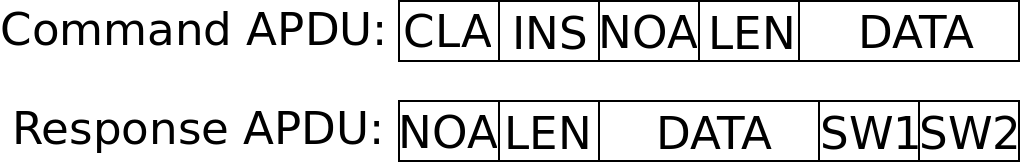
\includegraphics[width=1\hsize]{./images/myapdu.png}
\end{center}
\caption[Selbstdefinierter Dateninhalt der APDUs]{\label{myapdu}Selbstdefinierter Dateninhalt der APDUs}
\end{figure}

APDUs enthalten bis zu 256 Bytes, davon bis zu 252 Bytes für Daten.
Es sind ganze Trainingspläne und andere Objekte im Byte Format zwischen On-Card und Off-Card Teil zu übertragen. Dazu existiert pro Datenmodell in der dazugehörigen Klasse je eine Funktion zur Umwandlung von Instanz zu Byte Array und zur Erzeugung einer Instanz aus einem Byte Array. Diese Umwandlung  wurde eigens implementiert und orientiert sich am Aufbau von Ethernet Paketen. Ein Paket oder Byte Array besteht dabei immer aus einem Byte für einen eindeutigen Identifikator des Modells, zwei Bytes für die Anzahl der folgenden Bytes sowie Daten Bytes.
Eine Instanz des Modells MyDate mit den Attributen Jahr\footnote{Bei einem Jahr werden nur die letzten zwei Ziffern hexadezimal abgespeichert.}, Monat und Tag wird in folgendes Byte Repräsentation umgewandelt: $01$ $00$ $03$ $0e$ $07$ $0b$
\\

%verschlüsselung
Bei der Realisierung des Trainingssystemes werden keine Sicherheitsrelevanten Daten zwischen On-Card und Off-Card Teil übertragen. Auf Grund dessen wurde auf eine verschlüsselte Kommunikation mit asymmetrischer oder symmetrischer Verschlüsselung verzichtet.
Einzig Rollen-spezifische Schreibvorgänge sind in beiden Card Teilen durch je ein Passwort geschützt.
Der Trainer und der Sportler besitzen jeweils ein Passwort, welches mit der Java Bibliothek java.security.MessageDigest und derdarin enthaltenen  Hashfunktion SHA-256 zu einem 32 Byte langem Wert gehasht.
Dieser Hash ist auf der Smartcard gespeichert und muss bei der Anmeldung zum anschließenden Vergleich des Trainers oder Sportlers übertragen werden.
Der jeweilige Benutzer gibt in der grafischen Oberfläche sein Passwort im Klartext ein worauf die Programmlogik dieses hasht und es an die Smartcard überträgt.
Initial ist die Karte mit je einem Hash für Trainer und Sportler zu füllen. Im Zuge der Vereinfachung sind diese Werte bereits statisch gefüllt.
Um den Passworthash des Trainers zu setzen ist das in Listing \ref{lst:setpswds} dargestellte Kommando an die Smartcard zu senden.

\begin{lstlisting}[language=java, captionpos=b, caption=Setzen des Passwortes eines Sportlers in Form eines Kommandos, label=lst:setpswds]
/send 00 05 01 21 02 
\end{lstlisting}